\documentclass[fleqn,letterpaper]{article}
\usepackage{fullpage}
\usepackage[dvips]{graphicx}
\usepackage{amssymb}
\usepackage{fancyhdr}
\usepackage[active]{srcltx}
\addtolength{\parskip}{\baselineskip}
\pagestyle{fancy}
\headheight=12pt
\parindent 0cm

\begin{document}

\lhead{\it Instructor's Lab Manual for Physics 160 }
\cfoot{}
\rhead{\it Page \thepage~of \pageref{LastPage} }
\headsep=25pt
%\baselineskip=12pt

\section*{Boom Crane and Human Arm}

\subsection*{Additional Equipment}

\begin{itemize}
  \item{the board with drilled holes (and eyehooks) should be provided}
  \item{String is also provided (thicker than the stuff we hang weights off of the pulleys with)}
\end{itemize}

\subsection*{Objective}

This lab intends to build the student's skills with:
%
\begin{itemize}
 \item{Addition of Torques}
 \item{Understanding Newton's Second Law for rotation as applied to statics}
 \item{Estimating Uncertainties}
 \item{Using a fit to determine the velocity-dependence of the drag force}
\end{itemize}
%

\subsection*{Conceptual (C-level) (Done BEFORE Lab)}

The first bullet-point should be pretty straightforward for the students.  One new key point is that the students should draw the forces with the vector tails at the point of application on the object (so the weight is at the center of mass, the tension force is where the wire attaches to the beam, etc.).  

NOTE:  The ``Figure 1'' referred to was accidentally left out of the lab manual.  A reproduction of it was posted to D2L, and is reproduced here:

\begin{figure}[h!]
\centering
 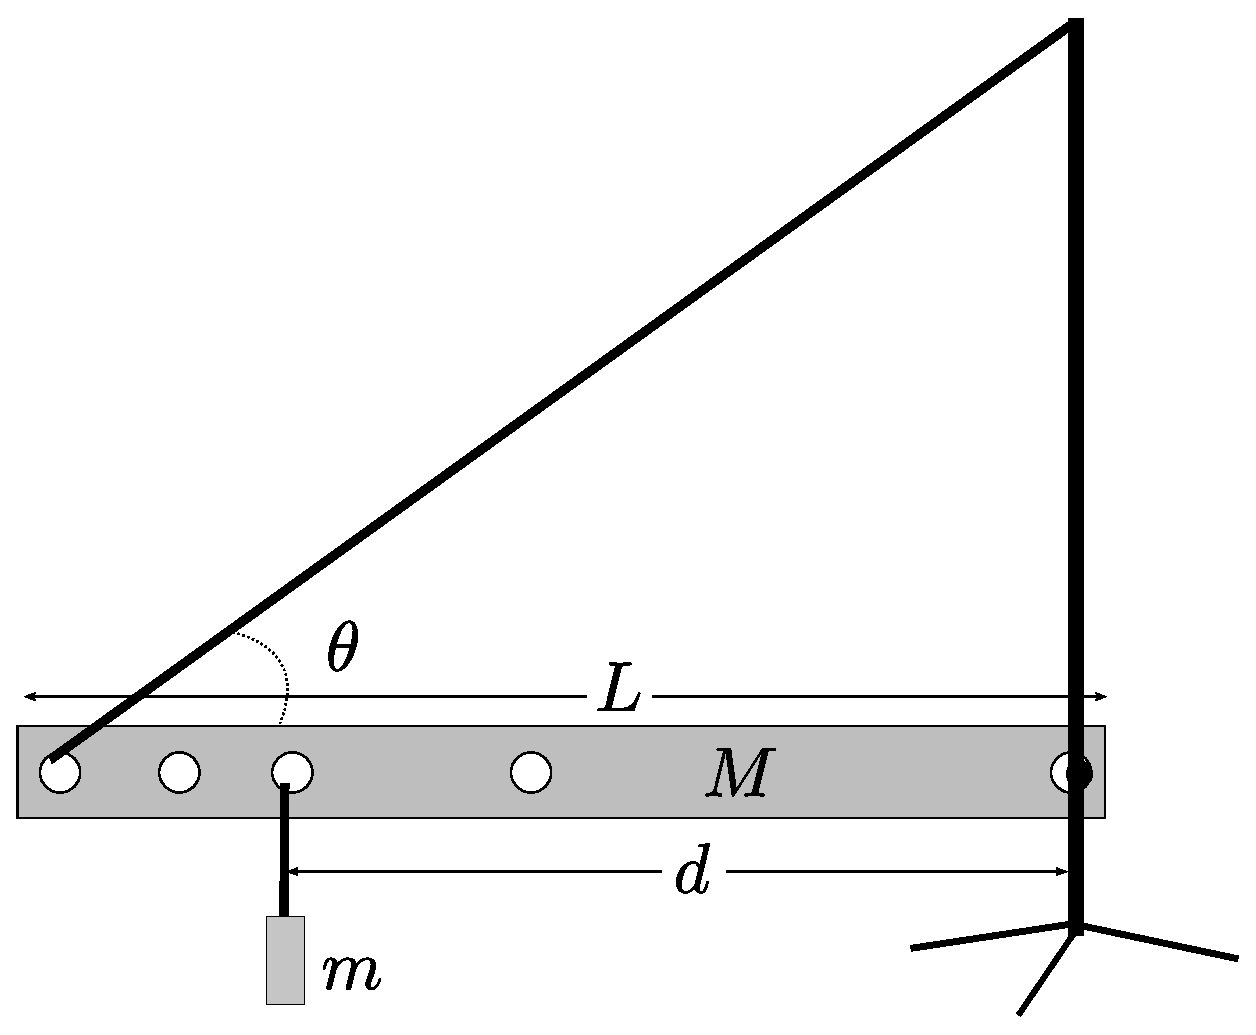
\includegraphics[height=45mm]{Figure1.eps}
\end{figure}


The second bullet-point where the students work out an equation for the tension in the supporting cable will be difficult for the students, since we have just started torque.  I am also attaching some hand-written notes that I posted for the students on adding torques, but for the purpose of teaching the lab, the highlights are:

\begin{itemize}
 \item{The torque $\vec{\tau}_F$ from a force $\vec{F}$ applied a distance $|\vec{r}|$ from the rotation axis at an angle $\phi$ has a magnitude given by
 \begin{equation}
  |\vec{\tau}_F| = |\vec{r}| |\vec{F}| \sin{\phi} = |\vec{r}| |\vec{F}_{\perp}|
 \end{equation}}
 \item{The sign of the torque is determined by the direction the torque \textbf{tries} to rotate the object: counter-clockwise is given a positive sign, and clockwise is given a negative sign.  Thus, in the figure above, the torque from the tension $\tau_T$ is negative, while the torque from both the hanging mass and the beam's center of mass is positive.}
 \item{The book does NOT talk about the right hand rule, OR about torques as being ``into'' or ``out of'' the page.  The students are NOT expected to know this.}
\end{itemize}

\subsubsection*{Quick Solution to C-Level}

Below is a very quick solution to the C-Level.  Here I assume that the CM is located at $L/2$ and that the tension is located at a distance $L$ from the pivot.  

\begin{eqnarray}
 I \alpha & = & \tau_T + \tau_m + \tau_M \\
 0 & = & -|\vec{F}_T| L \sin \phi + m g d \sin 90^{\circ} + M g \frac{L}{2} \sin 90^{\circ} \\
 |\vec{F}_T| L \sin \phi & = & m g d  + M g \frac{L}{2} \\
 |\vec{F}_T| & = & \frac{m g d  + M g \frac{L}{2}}{L \sin \phi} \\
 |\vec{F}_T| & = & g\frac{(m d/L  + M/2)}{\sin \phi}
\end{eqnarray}

If you instead use $d_T$ as the distance from the pivot to the tension and $d_M$ as the distance to the center of mass, you find:

\begin{equation}
 |\vec{F}_T| =  g\frac{(m d  + M d_M)}{d_T \sin \phi}
\end{equation}

In my test of the lab, this second equation was much more accurate, so the students will likely want to use this when completing the B-level, but they can use the ``simplified'' one above for the C-level on their first run-through.

\subsubsection*{Rubric}

\begin{itemize}
 \item{Pick a notebook at random from the group.  If the entire C-Level has not been attempted, dock 1 point from the group.}
 \item{If the students just ``quit'' or otherwise have a bad attitude are are not staying on task, dock a point (or two) after a warning.}
 \item{Other than these 2 things, assist the groups by asking leading questions as you see fit so they understand the C-level.  If they came prepared, worked hard, and got through the C-level, they get 4/4.}
\end{itemize}


\subsection*{Basic Lab (B-level)}

This is pretty straightforward: students will hang masses and measure the tension produced (with uncertainty), comparing with their prediction (with uncertainty).

Some additional notes:

\begin{itemize}
\item{Students should use the 100 g mass.  The 200 g one could also work for the B-level, but if they do the ``Human Arm'' A-Level, using the 200 g mass seemed unstable.  They are, however, free to \textit{try} any mass they choose.  This is for your reference as instructors.}
\item{Students may need to measure where the center of mass of the beam is.  The easiest way to do this is to find out where the beam is balanced.}
\item{The string used as the supporting cable is a bit stretchy.  This doesn't have too much of an impact on the B-Level, but it does on the A-level due to the higher tension in the string.  Depending on how much the beam ``dips'' below the horizontal, students should try to account for this in their uncertainty analysis.}
\item{UNCERTAINTIES -- This can be difficult since we don't really do explicit uncertainty propagation in this class.  However, students can obtain a reasonable estimate using the following procedure:
  \begin{itemize}
  \item{Estimate the uncertainty $\sigma$ in a measured quantity (say $d$)}
  \item{Compute their ``prediction'' for the tension with both $d + \sigma_d$ and $d - \sigma_d$ to get a ``high'' and ``low'' estimate for the tension.}
  \item{Divide the range (``high'' - ``low'') by 2, this will give an estimate of the uncertainty in the tension.}
  \item{Students can repeat if needed for other quantities (such as angles, masses, other positions, etc.)}
  \end{itemize}}
\end{itemize}

\subsubsection*{Rubric -- Lab Summary}

There should be a single plot that the students submit (tension vs $d$) with two data sets: their calculated (predicted) tensions, and the measured tensions (both vs $d$).

For this lab, specifically, they should have:

\begin{enumerate}
 \item{
  \begin{itemize}
   \item{Some diagrams and numbers present, very minimal.}
  \end{itemize}
}
 \item{
  \begin{itemize}
   \item{Plot of tension vs. $d$ present, including labels and units}
   \item{Some uncertainties missing}
   \item{Reported results, but no interpretation}
  % \item{No mention of the scale used}
  \end{itemize}
}
 \item{
  \begin{itemize}
 %  \item{Stating what scale they used}
   \item{All uncertainties present}
   \item{Linear fit present on the plot}
 %  \item{Two methods to determine uncertainties}
   \item{Some physics, but no explicit mention of the model used to fit the drag vs velocity plot (missing ``we expected it to be linear since $|\vec{F}_T| = g\frac{(m d  + M d_M)}{d_T \sin \phi}$, so it is linear in $d$'')}
  \end{itemize}
}
 \item{
  \begin{itemize}
   \item{Explicit mention of $|\vec{F}_T| = g\frac{(m d  + M d_M)}{d_T \sin \phi}$}
   \item{Discussion of how they obtained the uncertainties.}
  \end{itemize}
}
\end{enumerate}


\subsection*{Advanced/Extended Lab Ideas (A-level)}

Students may pick a single A-level to do.  They do not need to stay with their in-class group (though many choose to).

\begin{itemize}
 \item{The first A-level suggests that they modify their setup to model a human arm.  They would attach the supporting string to the eyehook nearest the pivot, and repeat the analysis of the B-Level.  They should find that the tension is much higher, due to the shorter distance from the pivot.}
\end{itemize}

\subsubsection*{Rubric -- Lab Summary}

Follow the rubric on page 7 of the lab manual.  Since the students can choose any A-level, I won't be writing up a detailed rubric for every suggestion.  Hopefully, the B-level rubrics included here help to establish a good guideline.  If you have further questions, please ask!

\label{LastPage}

\end{document}